% ------------------------------------------------------------------------------
% TYPO3 CMS 8.5 - What's New - Chapter "In-Depth Changes" (Italian Version)
%
% @author	Michael Schams <schams.net>
% @license	Creative Commons BY-NC-SA 3.0
% @link		http://typo3.org/download/release-notes/whats-new/
% @language	English
% ------------------------------------------------------------------------------
% LTXE-CHAPTER-UID:		5ebcecbe-66abfa57-cf38bc00-aa637965
% LTXE-CHAPTER-NAME:	In-Depth Changes
% ------------------------------------------------------------------------------

\section{Modifiche rilevanti}
\begin{frame}[fragile]
	\frametitle{Modifiche rilevanti}

	\begin{center}\huge{Capitolo 3:}\end{center}
	\begin{center}\huge{\color{typo3darkgrey}\textbf{Modifiche rilevanti}}\end{center}

\end{frame}

% ------------------------------------------------------------------------------
% LTXE-SLIDE-START
% LTXE-SLIDE-UID:		89b8e3eb-3a9f062e-d4aef361-d0ffce14
% LTXE-SLIDE-ORIGIN:	bde270e6-ffef8544-ea472ed5-89ba8c3d English
% LTXE-SLIDE-TITLE:		#78581: FormEngine Data Providers
% ------------------------------------------------------------------------------

\begin{frame}[fragile]
	\frametitle{Modifiche rilevanti}
	\framesubtitle{FormEngine Data Providers}

	\begin{itemize}
		\item Il FormEngine data provider \texttt{TcaFlexFetch} è stato unito in \texttt{TcaFlexPrepare}
		\item Questo riguarda solamente le situazioni, improbabili, in cui un "data provider" 
			personalizzato ha dichiarato una dipendenza da \texttt{TcaFlexFetch}
	\end{itemize}

\end{frame}

% ------------------------------------------------------------------------------
% LTXE-SLIDE-START
% LTXE-SLIDE-UID:		878fc955-e8ac383a-8651719d-11c28425
% LTXE-SLIDE-ORIGIN:	f0fb603c-54e9f255-03140395-b6b18103 English
% LTXE-SLIDE-TITLE:		#78384: Frontend ignores TCA in ext_tables.php
% ------------------------------------------------------------------------------
\begin{frame}[fragile]
	\frametitle{Modifiche rilevanti}
	\framesubtitle{TCA in \texttt{ext\_tables.php}}

	\begin{itemize}
		\item Le richieste di frontend non caricano più il file \texttt{ext\_tables.php}
		\item Questa modifica ha un impatto sulle estensioni che configurano TCA in \texttt{ext\_tables.php}\newline
			\small(che non è permesso in ogni caso)\normalsize
		\item Install Tool dispone di un test "TCA ext\_tables check" per identificare queste estensioni
	\end{itemize}

	\begin{figure}
		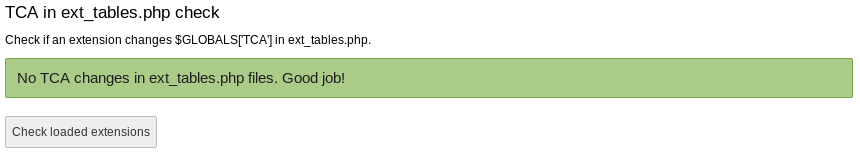
\includegraphics[width=0.95\linewidth]{InDepthChanges/78384-install-tool-tca-in-exttables-check.png}
	\end{figure}

\end{frame}
% ------------------------------------------------------------------------------
% LTXE-SLIDE-START
% LTXE-SLIDE-UID:		68b40200-670e6490-2e833717-f989d6a0
% LTXE-SLIDE-ORIGIN:	bdcd2449-b679717b-9f23eb32-018953b4 English
% LTXE-SLIDE-TITLE:		#78191: Remove support for transForeignTable/transOrigPointerTable in TCA
% ------------------------------------------------------------------------------
\begin{frame}[fragile]
	\frametitle{Modifiche rilevanti}
	\framesubtitle{TCA in \texttt{ext\_tables.php}}

	\begin{itemize}
		\item Le tabelle del database che contenevano record localizzati e tradotti erano gestiti nel TCA

			\begin{itemize}
				\item \texttt{\$TCA[<table\_name>]['ctrl']['transForeignTable']}\newline
					(usually pointed to table: \texttt{pages\_language\_overlay})
				\item \texttt{\$TCA[<table\_name>]['ctrl']['transOrigPointerTable']}\newline
					(usually pointed to table: \texttt{pages})
			\end{itemize}

		\item Questa configurazione è stata sostituita con i nomi di tabella del core, al fine di evitare una	
			gestione particolare e prepararsi ad un unione di entrambe le tabelle in un futuro

	\end{itemize}

\end{frame}

% ------------------------------------------------------------------------------
% LTXE-SLIDE-START
% LTXE-SLIDE-UID:		0243c764-0b3c2d89-2b5967a0-743b4a29
% LTXE-SLIDE-ORIGIN:	ede02440-cafd3417-eb416f09-8e024ef2 English
% LTXE-SLIDE-TITLE:		#78383: Tables removed from defaultCategorizedTables
% ------------------------------------------------------------------------------
\begin{frame}[fragile]
	\frametitle{Modifiche rilevanti}
	\framesubtitle{Tabelle rimosse da \texttt{defaultCategorizedTables}}

	\begin{itemize}
		\item Le seguenti tabelle sono state rimosse da \texttt{defaultCategorizedTables}:

			\begin{itemize}
				\item \texttt{pages}
				\item \texttt{tt\_content}
				\item \texttt{sys\_file\_metadata}
			\end{itemize}

		\item Per queste tabelle le API del core\newline
			\texttt{ExtensionManagementUtility::makeCategorizable()}\newline
			sono eseguite per determinare una posizione comune del campo di categoria

	\end{itemize}

\end{frame}


% ------------------------------------------------------------------------------
% LTXE-SLIDE-START
% LTXE-SLIDE-UID:		13a6cf6b-e9e29ef3-2f7c0459-2f186e7a
% LTXE-SLIDE-ORIGIN:	dd31e5d5-ca09ae5e-eb87d926-0ffe8f0a English
% LTXE-SLIDE-TITLE:		Low-level parameters changes (1)
% ------------------------------------------------------------------------------
\begin{frame}[fragile]
	\frametitle{Modifiche rilevanti}
	\framesubtitle{Cambio dei parametri a basso livello (1)}

	% changes: #78417, #78439, #78520, #78552, #78577, #78623, #78627 and #78895

	\begin{itemize}
		\item I comandi a basso livello elencati di seguito usano ora la Symfony Console 
		\item I nuovi comandi si comportano come quelli vecchi, ma permettono l'uso di alcuni parametri

			\begin{itemize}
				\item \texttt{DeletedRecordsCommand}
				\item \texttt{CleanFlexFormsRecordsCommand}
				\item \texttt{OrphanRecordsCommand}
				\item \texttt{LostFilesCommand}
				\item \texttt{MissingFilesCommand}
				\item \texttt{MissingRelationsCommand}
				\item \texttt{DoubleFilesCommand}
				\item \texttt{RteImagesCommand}
			\end{itemize}

	\end{itemize}

\end{frame}



% ------------------------------------------------------------------------------
% LTXE-SLIDE-START
% LTXE-SLIDE-UID:		964bd97f-4a4bb87b-ef161451-4d02e765
% LTXE-SLIDE-ORIGIN:	3a9d25bb-d948368d-e2a92666-6170eaad English
% LTXE-SLIDE-TITLE:		Low-level parameters changes (2)
% ------------------------------------------------------------------------------
\begin{frame}[fragile]
	\frametitle{Modifiche rilevanti}
	\framesubtitle{Cambio dei parametri a basso livello (2)}

	% changes: #78417, #78439, #78520, #78552, #78577, #78623, #78627 and #78895

	\begin{itemize}
		\item Le classi PHP correlate sono state rimosse\newline
			\smaller(e.g. \texttt{TYPO3\textbackslash
				CMS\textbackslash
				Lowlevel\textbackslash
				DeletedRecordsCommand})
			\normalsize

		\item L'esecuzione dei comandi via \texttt{cli\_dispatch} non funziona più\newline
			\smaller(es. \texttt{typo3/cli\_dispatch lowlevel cleaner deleted})\normalsize
		\item La chiamata alla classe PHP restituisce ora un errore PHP fatale

		\item I comandi possono essere eseguiti via CLI come di seguito:\newline
			\smaller\texttt{/typo3/sysext/core/bin/typo3 cleanup:<command>}\normalsize\newline
			per esempio:\newline
			\smaller\texttt{/typo3/sysext/core/bin/typo3 cleanup:deletedrecords}\normalsize

	\end{itemize}

\end{frame}




% ------------------------------------------------------------------------------
% LTXE-SLIDE-START
% LTXE-SLIDE-UID:		7ea457b4-c861a628-c2622049-881bbe22
% LTXE-SLIDE-ORIGIN:	ec6817fd-c3364ffb-c74e9523-a18a3095 English
% LTXE-SLIDE-TITLE:		Re-factor FlexForm Data Structure Handling
% ------------------------------------------------------------------------------
\begin{frame}[fragile]
	\frametitle{Modifiche rilevanti}
	\framesubtitle{Re-factor FlexForm Data Structure Handling}

	% https://forge.typo3.org/issues/78581
	% https://forge.typo3.org/issues/78616
	% https://forge.typo3.org/issues/78852
	% https://forge.typo3.org/issues/69715

	\begin{itemize}
		\item Con il deprecamento di \texttt{BackendUtility::getFlexFormDS()} l'hook
			\texttt{getFlexFormDSClass} non è più richiamato

	\end{itemize}

\end{frame}





% ------------------------------------------------------------------------------
% LTXE-SLIDE-START
% LTXE-SLIDE-UID:		f313616e-0417658b-5a8bfcc3-b23e9e5f
% LTXE-SLIDE-ORIGIN:	b400c3b8-3e402480-cd7d6ff3-96cd93aa English
% LTXE-SLIDE-TITLE:		#76085: Add fluid debug information to admin panel
% ------------------------------------------------------------------------------
\begin{frame}[fragile]
	\frametitle{Modifiche rilevanti}
	\framesubtitle{Admin Panel}

	\begin{itemize}
		\item Admin Panel ha una nuova funzionalità per impostare il debug dell'output di Fluid:\newline
			\textbf{Preview -> Mostra debug di fluid}
		\item Se attivo, i seguenti dettagli sono mostrati nel frontend:

			\begin{itemize}
				\item path del file di template di un partial
				\item nome della sezione
			\end{itemize}

		\item Questa funzione permette agli integratori di individuare facilmente il template e la sezione corrette

	\end{itemize}

\end{frame}






% ------------------------------------------------------------------------------
% LTXE-SLIDE-START
% LTXE-SLIDE-UID:		8719b86a-e28321ff-6d080e92-f8afd6f2
% LTXE-SLIDE-ORIGIN:	60a2d39f-f04b8bf1-dc758912-607ed07e English
% LTXE-SLIDE-TITLE:		#52286: System Status Updates Report via email
% ------------------------------------------------------------------------------
\begin{frame}[fragile]
	\frametitle{Modifiche rilevanti}
	\framesubtitle{Stato degli aggiornamenti di sistema (Report)}

	\begin{itemize}
		\item I risultati dei test di "Stato degli aggiornamenti di sistema (report)" può essere inviato via email
		\item Un checkbox è stato aggiunto alla configurazione per:

			\begin{itemize}
				\item inviare una mail se il sistema riscontra un avviso o un errore
				\item generare sempre una email
			\end{itemize}

		\item Di default include solo avvisi e errori

	\end{itemize}

\end{frame}







% ------------------------------------------------------------------------------
% LTXE-SLIDE-START
% LTXE-SLIDE-UID:		e8af7d05-ff4a3d9d-2b7f4473-474577cb
% LTXE-SLIDE-ORIGIN:	e4e2ead3-c07beb21-e8100580-d0e7c756 English
% LTXE-SLIDE-TITLE:		#58637: Purge language packs in language module
% ------------------------------------------------------------------------------
\begin{frame}[fragile]
	\frametitle{Modifiche rilevanti}
	\framesubtitle{Pacchetto Linguaggi}

	\begin{itemize}
		\item Disattivando delle lingue nel modulo "Languages" lascia le lingue rimanenti
			nella directory \texttt{typo3conf/l10n/<locale>/}
		\item Un bottone "rimuovi" è stato aggiunto, per disabilitare le lingue e pulire i
			dati nella directory
	\end{itemize}

\end{frame}








% ------------------------------------------------------------------------------
% LTXE-SLIDE-START
% LTXE-SLIDE-UID:		6cb70a13-1667e4ad-8a77aea2-4c246363
% LTXE-SLIDE-ORIGIN:	08961fb3-00cbc9f4-964f8d01-6e59e782 English
% LTXE-SLIDE-TITLE:		#67909: Hook added to localize() function
% ------------------------------------------------------------------------------
\begin{frame}[fragile]
	\frametitle{Modifiche rilevanti}
	\framesubtitle{Hook in DataHandler \texttt{localize()}}

	% decrease font size for code listing
	\lstset{basicstyle=\tiny\ttfamily}

	\begin{itemize}
		\item Un nuovo hook è stato aggiunto alla funzione \texttt{localize()}
		\item Questo permette ad esempio di usare un servizio di traduzione esterno o funzioni personalizzate
			di traduzione che gestiscono differenti trasformazioni del contenuto
	\end{itemize}

	\begin{itemize}
		\item Hook:\newline
			\smaller
				\texttt{\$GLOBALS['TYPO3\_CONF\_VARS']['SC\_OPTIONS']\newline
				\tabto{0.4cm}['t3lib/class.t3lib\_tcemain.php']['processTranslateToClass']}
			\normalsize

		\item Esempio d'uso:

			\begin{lstlisting}
				class YourHookClass
				{
				  public function processTranslateTo_copyAction(&$content, $lang, $dataHandler)
				  {
				    // Fai qualcosa con il contenuto (traduzione, alterazioni, etc.)
				  }
				}
			\end{lstlisting}
	\end{itemize}

\end{frame}









% ------------------------------------------------------------------------------
% LTXE-SLIDE-START
% LTXE-SLIDE-UID:		1c102e30-9765f656-226c4b7e-294eab90
% LTXE-SLIDE-ORIGIN:	8b1a9661-d6fab90f-9c856224-ee663aa2 English
% LTXE-SLIDE-TITLE:		#77757: Re-check if an UpdateWizard should run
% ------------------------------------------------------------------------------
\begin{frame}[fragile]
	\frametitle{Modifiche rilevanti}
	\framesubtitle{Update Wizard}

	\begin{columns}[T]
		\begin{column}{.5\textwidth}
			il wizard di update nell'Install Tool elenca tutte le attività segnate come \textit{completate}.
			\newline\newline
			Un checbox e un bottone "Riverifica i check scelti" permettono di rifare gli aggiornamenti.
			Il wizard verifica se ci sono attività da eseguire nuovamente.
		\end{column}
		\begin{column}{.5\textwidth}
			\begin{figure}\vspace*{-0.5cm}
				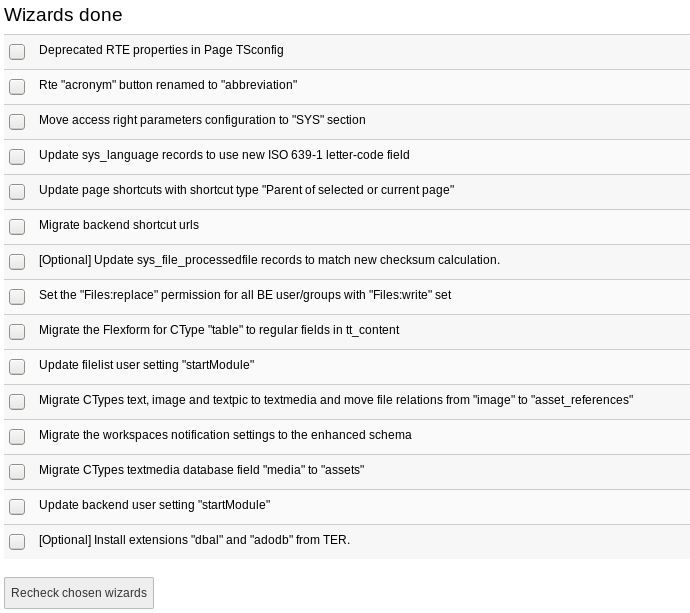
\includegraphics[width=0.8\linewidth]{InDepthChanges/77757-upgrade-wizard.png}
			\end{figure}
		\end{column}
	\end{columns}

\end{frame}









% ------------------------------------------------------------------------------
% LTXE-SLIDE-START
% LTXE-SLIDE-UID:		c4c6e6d8-01f81e42-78bae867-a2773acc
% LTXE-SLIDE-ORIGIN:	94640f3d-0f632507-a2166719-5adc755e English
% LTXE-SLIDE-TITLE:		#78523: Suggest wizard provides option to define ordering of results
% ------------------------------------------------------------------------------
\begin{frame}[fragile]
	\frametitle{Modifiche rilevanti}
	\framesubtitle{Suggest Wizard}

	% decrease font size for code listing
	\lstset{basicstyle=\tiny\ttfamily}

	\begin{itemize}
		\item Il FormEngine ("TCEforms") permette di configurare l'ordine dei risultati del "suggest wizard"
		\item La nuova opzione è una definizione standard di SQL order-by:\newline
			\small\texttt{'orderBy' => 'field ASC/DESC'}\normalsize
		\item Esempio di configurazione TCA:

			\begin{lstlisting}
				'config' => [
				  ...
				  'wizards' => [
				    'suggest' => [
				      'type' => 'suggest',
				      'default' => [
				        'searchWholePhrase' => true,
				        'addWhere' => ' AND tx_news_domain_model_news.uid != ###THIS_UID###',
				        'orderBy => 'datetime DESC',
				      ]
				    ],
				  ],
				]
			\end{lstlisting}

	\end{itemize}

\end{frame}











% ------------------------------------------------------------------------------
% LTXE-SLIDE-START
% LTXE-SLIDE-UID:		8dc1db5e-e56dc460-9bfec57c-4c69cadd
% LTXE-SLIDE-ORIGIN:	0907e5d3-a12751cb-23f49488-7a05a208 English
% LTXE-SLIDE-TITLE:		Miscellaneous
% ------------------------------------------------------------------------------
\begin{frame}[fragile]
	\frametitle{Modifiche rilevanti}
	\framesubtitle{Varie}

	% #78103: Add missing information status for addSystemMessage
	% #78575: Get enumeration constants
	% #75232: Spread TypeConverter priorities

	\begin{itemize}
		\item Tutte le informazioni di sistema aggiunte da \texttt{addSystemInformation()} hanno
			ora come valore di default \texttt{InformationStatus::STATUS\_NOTICE}
		\item Le costanti Enumeration possono ora essere recuperate facilmente:

			\begin{itemize}
				\item \texttt{EnumerationClass::getName(\$value);}
				\item \texttt{EnumerationClass::getHumanReadableName(\$value);}
			\end{itemize}

		\item Le priorità del core TypeConverters sono cambiate da 
			\texttt{1}, \texttt{2}, \texttt{3},...\newline a \texttt{10}, \texttt{20}, \texttt{30},...
			Al momento della registrazione di TypeConverter(s) personalizzati, assicurarsi che stiano utilizzano le priorità corrette.

		\item \href{https://en.wikipedia.org/wiki/ISO_8601}{ISO-8601} è utilizzato per passare i valori di data e datetime tra server
			e client. Verificare se i vostri FormEngine personalizzati renderizzano i tipi in modo aggiornato (\texttt{eval=date/datetime}).

	\end{itemize}

\end{frame}












% ------------------------------------------------------------------------------
